\begin{appendices}
\chapter{Exercise 1}
\section{Q1}
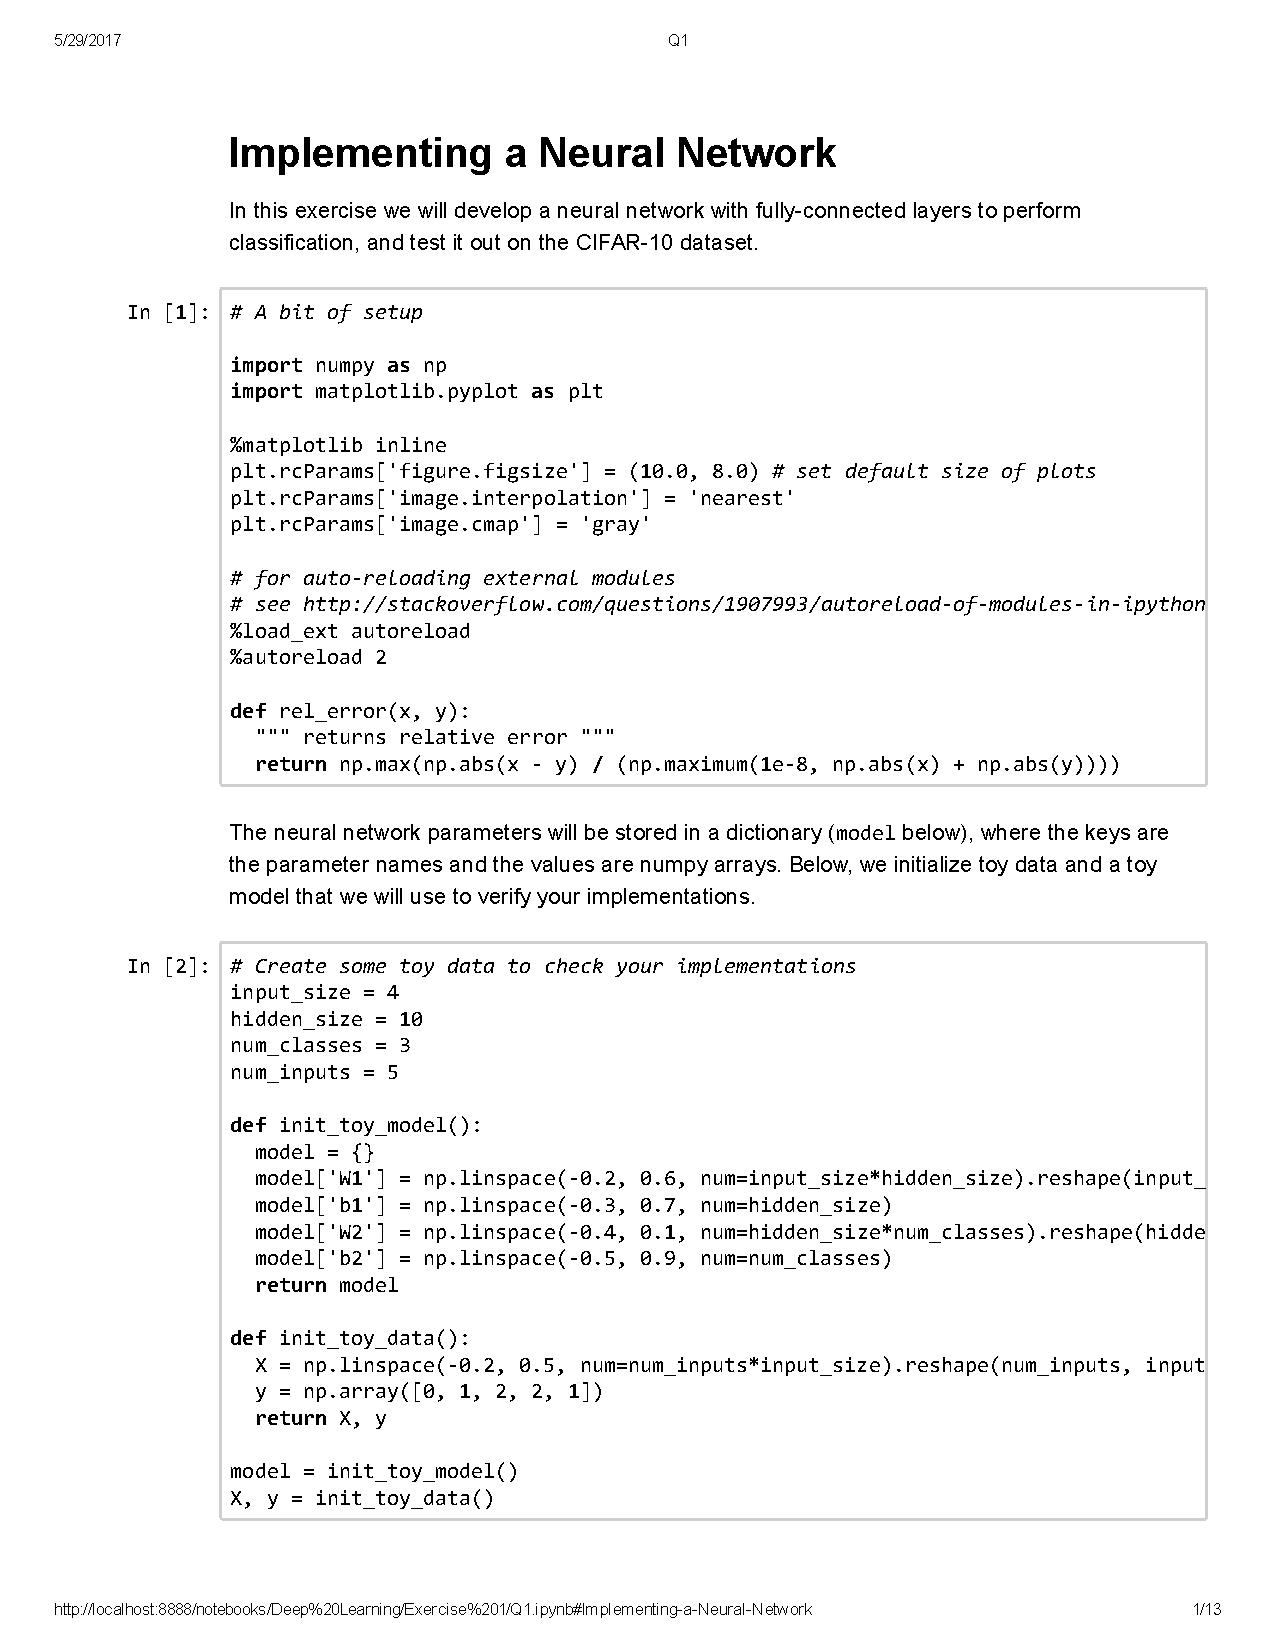
\includepdf[pages=-]{../chapter/appendix/Exercise1/Q1}
\section{Q2}
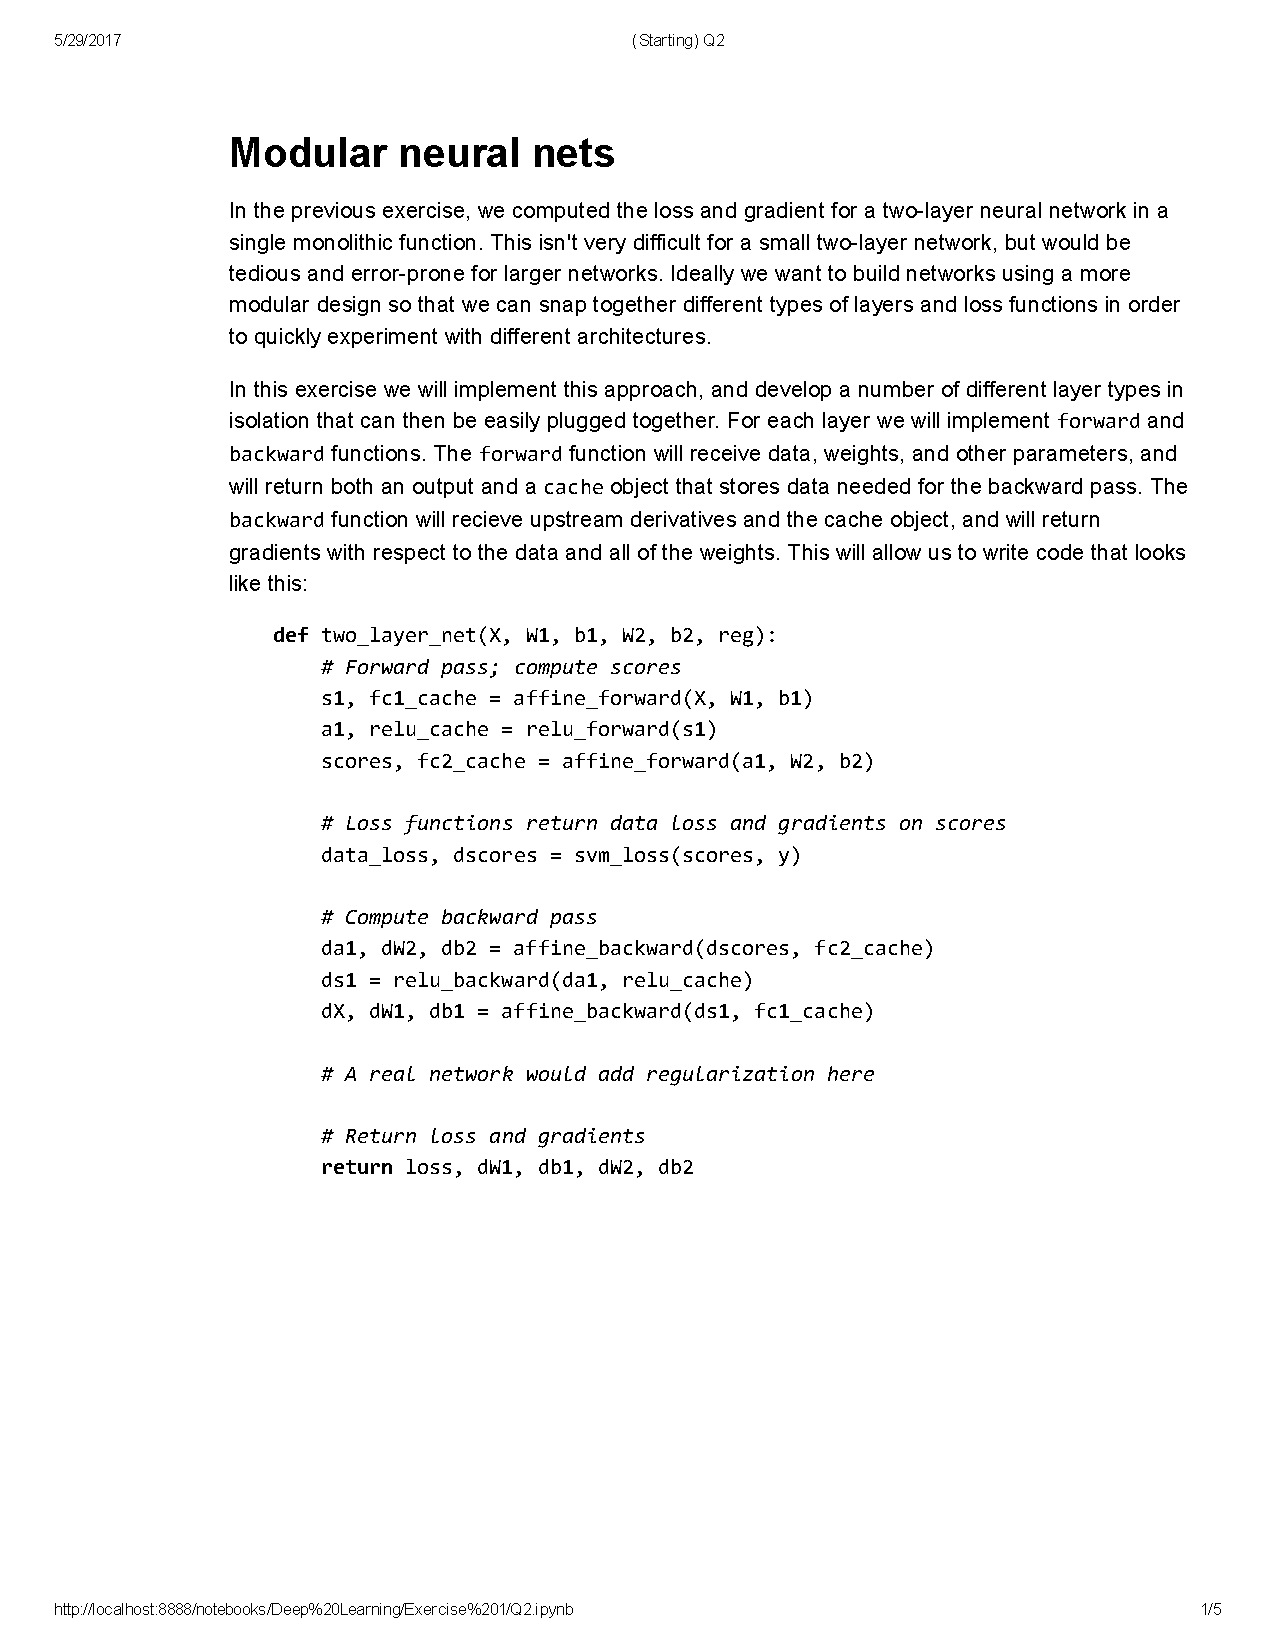
\includepdf[pages=-]{../chapter/appendix/Exercise1/Q2}
\section{Code}
\subsection{neural\_net.py}
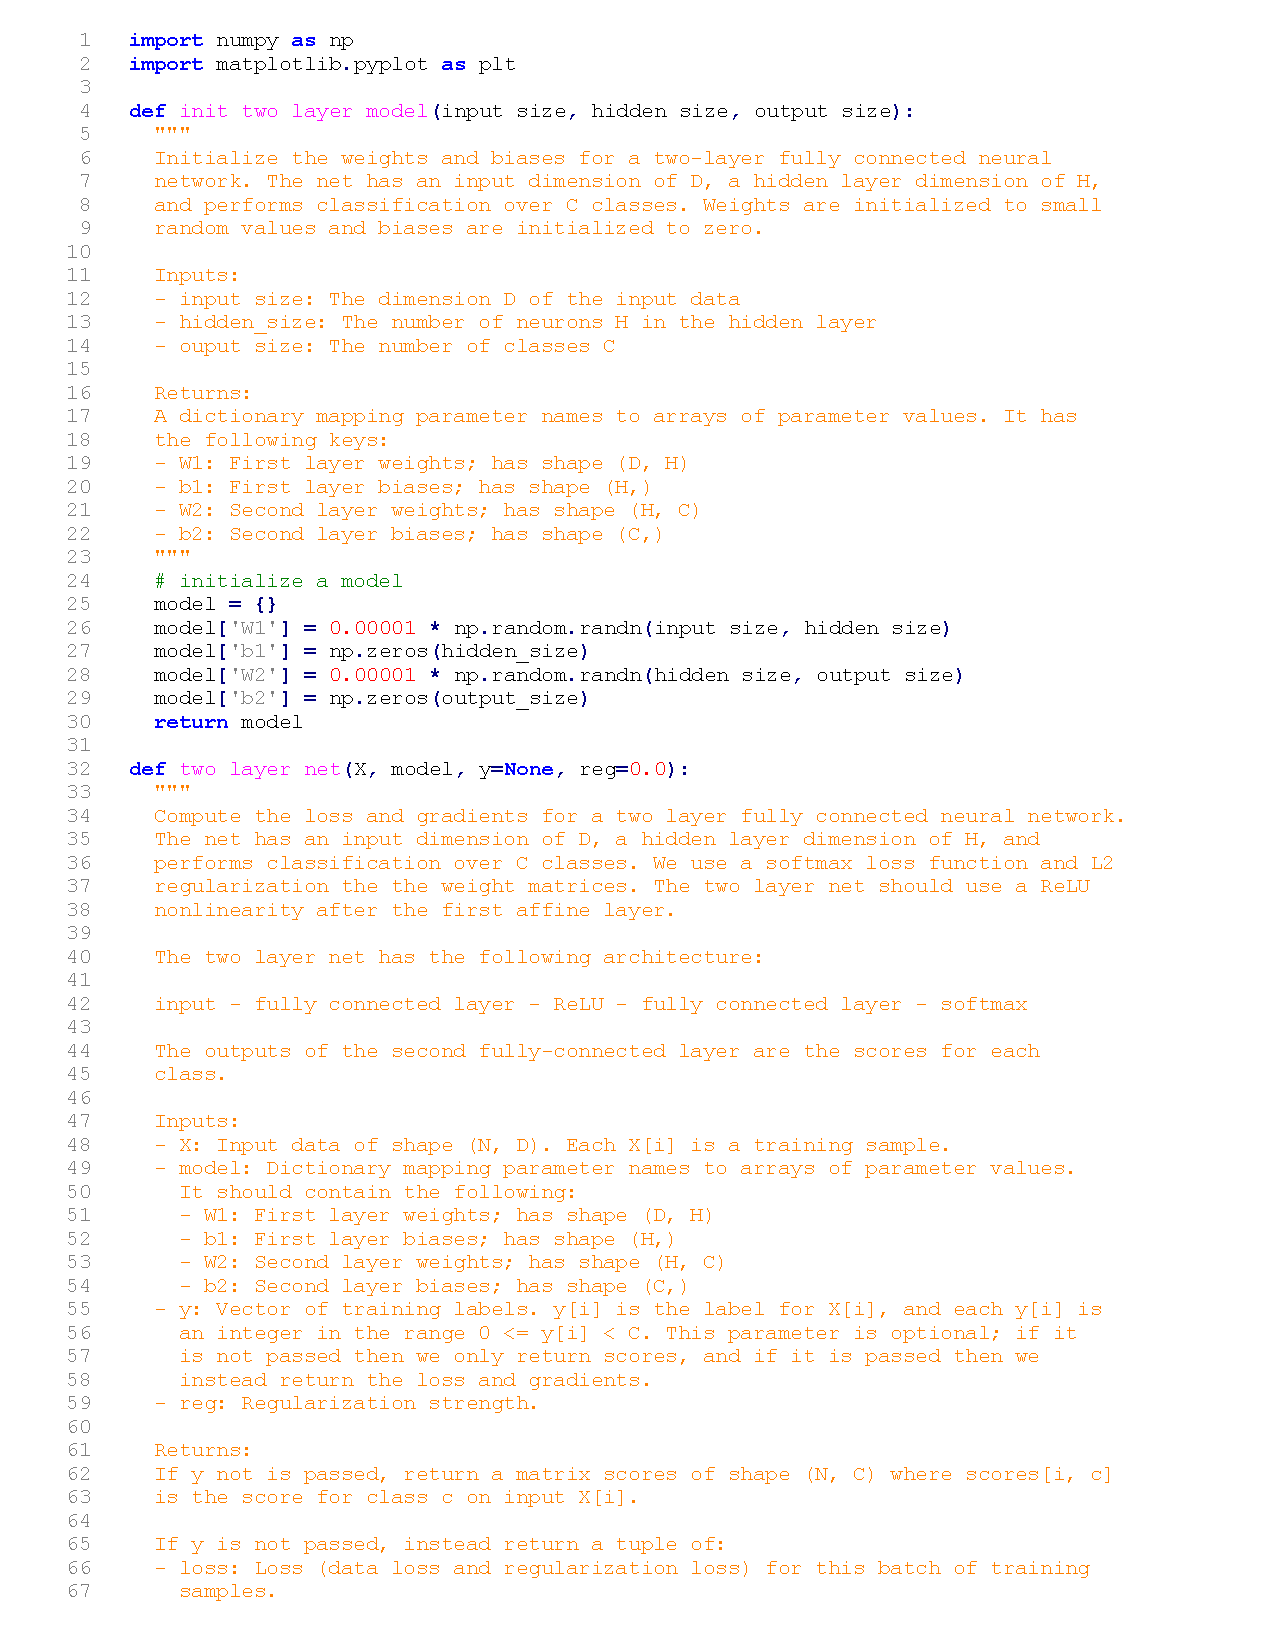
\includepdf[pages=-]{../chapter/appendix/Exercise1/neural_net}
\subsection{layers.py}
\includepdf[pages=-]{../chapter/appendix/Exercise1/layers}
\end{appendices}

\begin{appendices}
\chapter{Exercise 2}
\section{Q1}
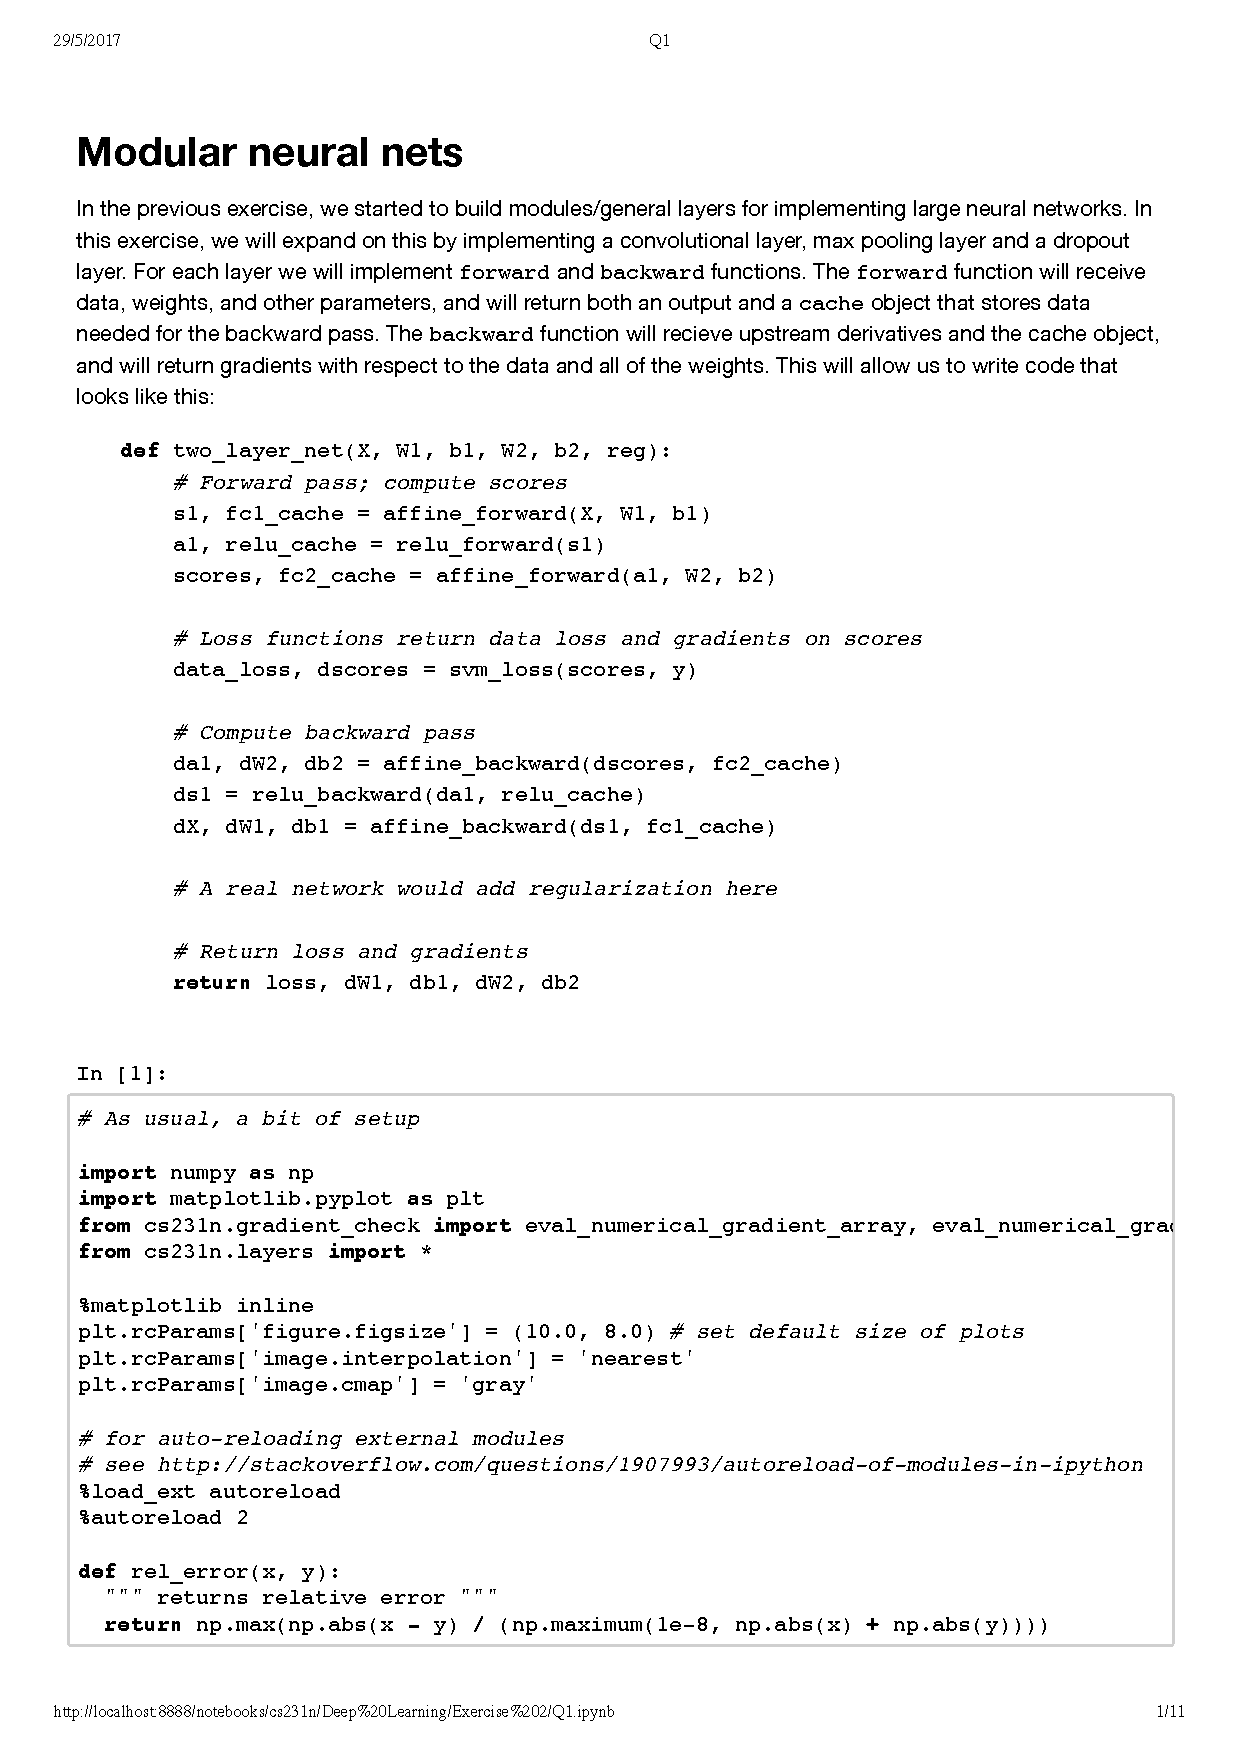
\includepdf[pages=-]{../chapter/appendix/Exercise2/Q1}
\section{Q2}
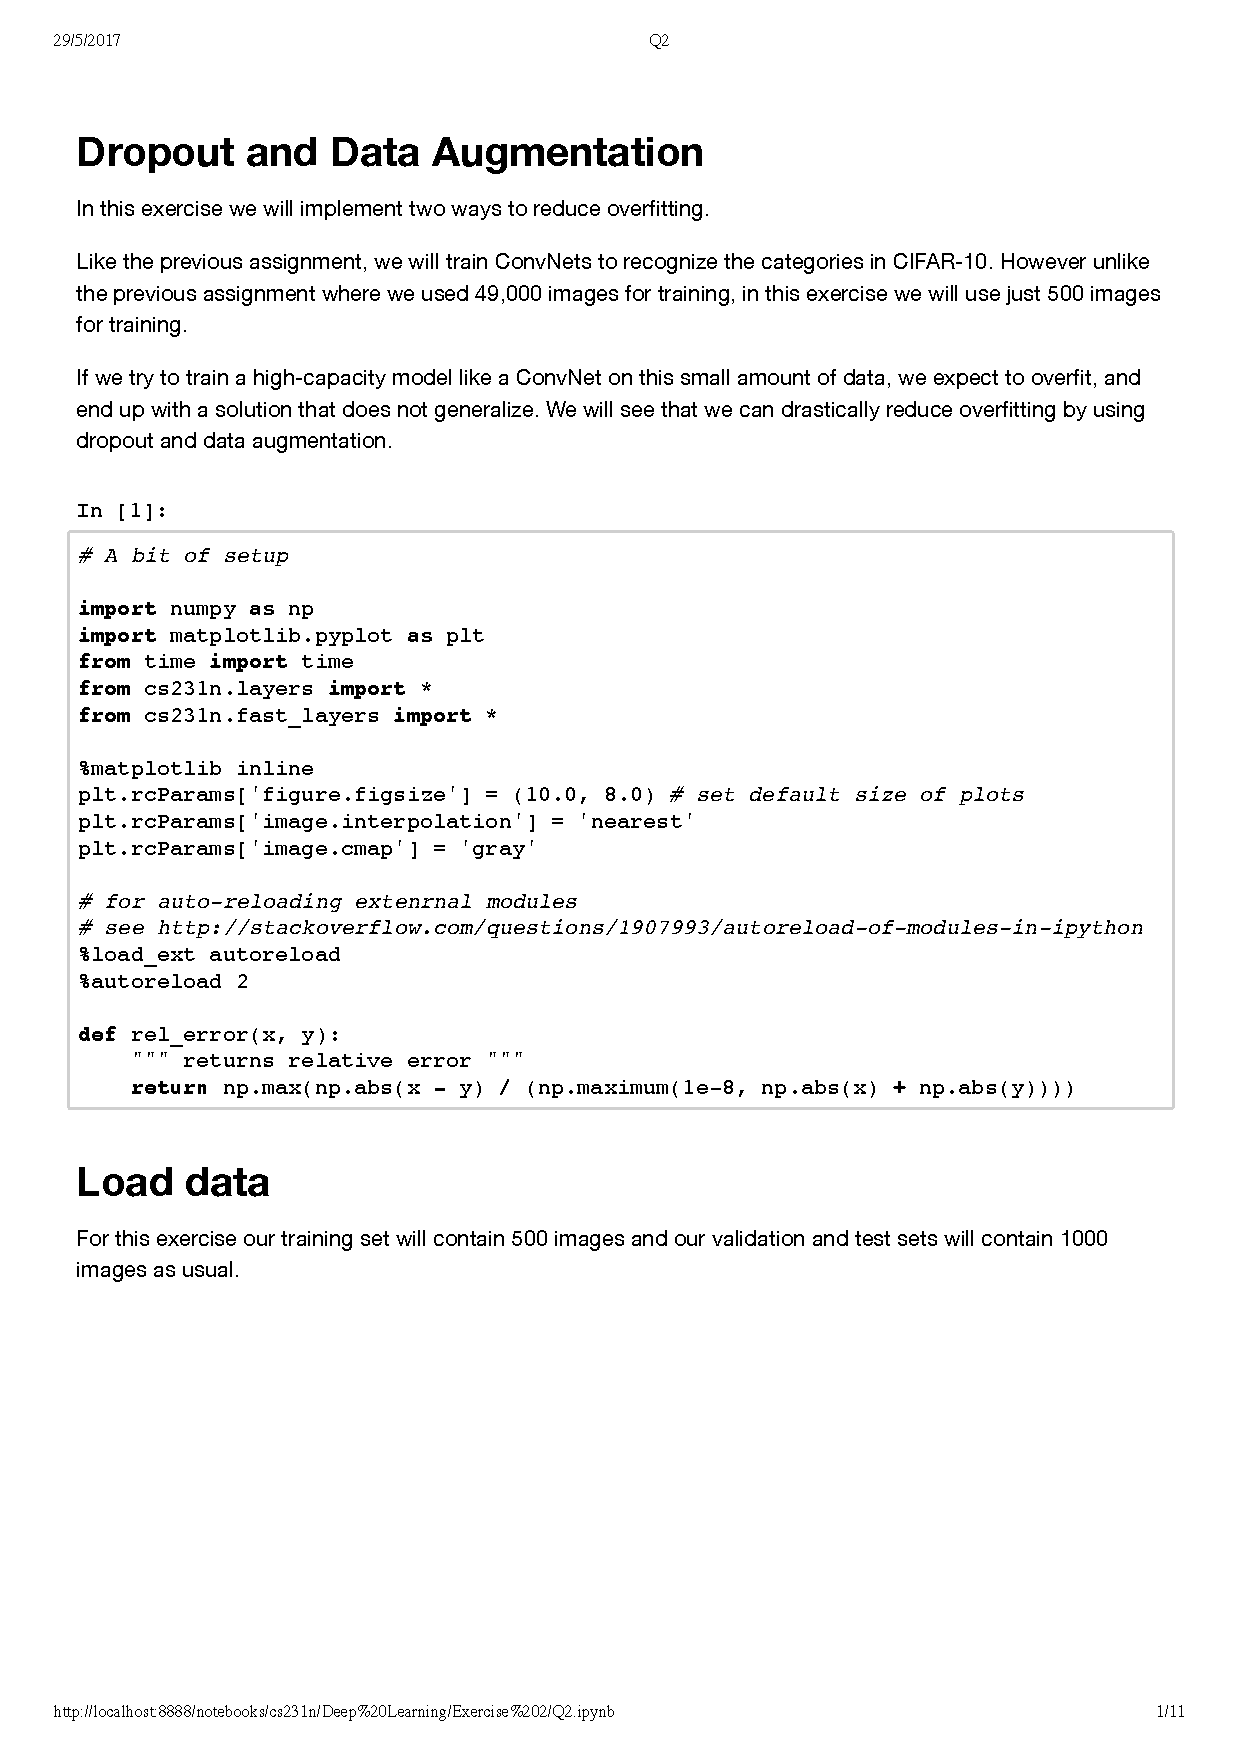
\includepdf[pages=-]{../chapter/appendix/Exercise2/Q2}
\section{Code}
\subsection{layers.py}
\includepdf[pages=-]{../chapter/appendix/Exercise2/layers}
\subsection{data\_augmentation.py}
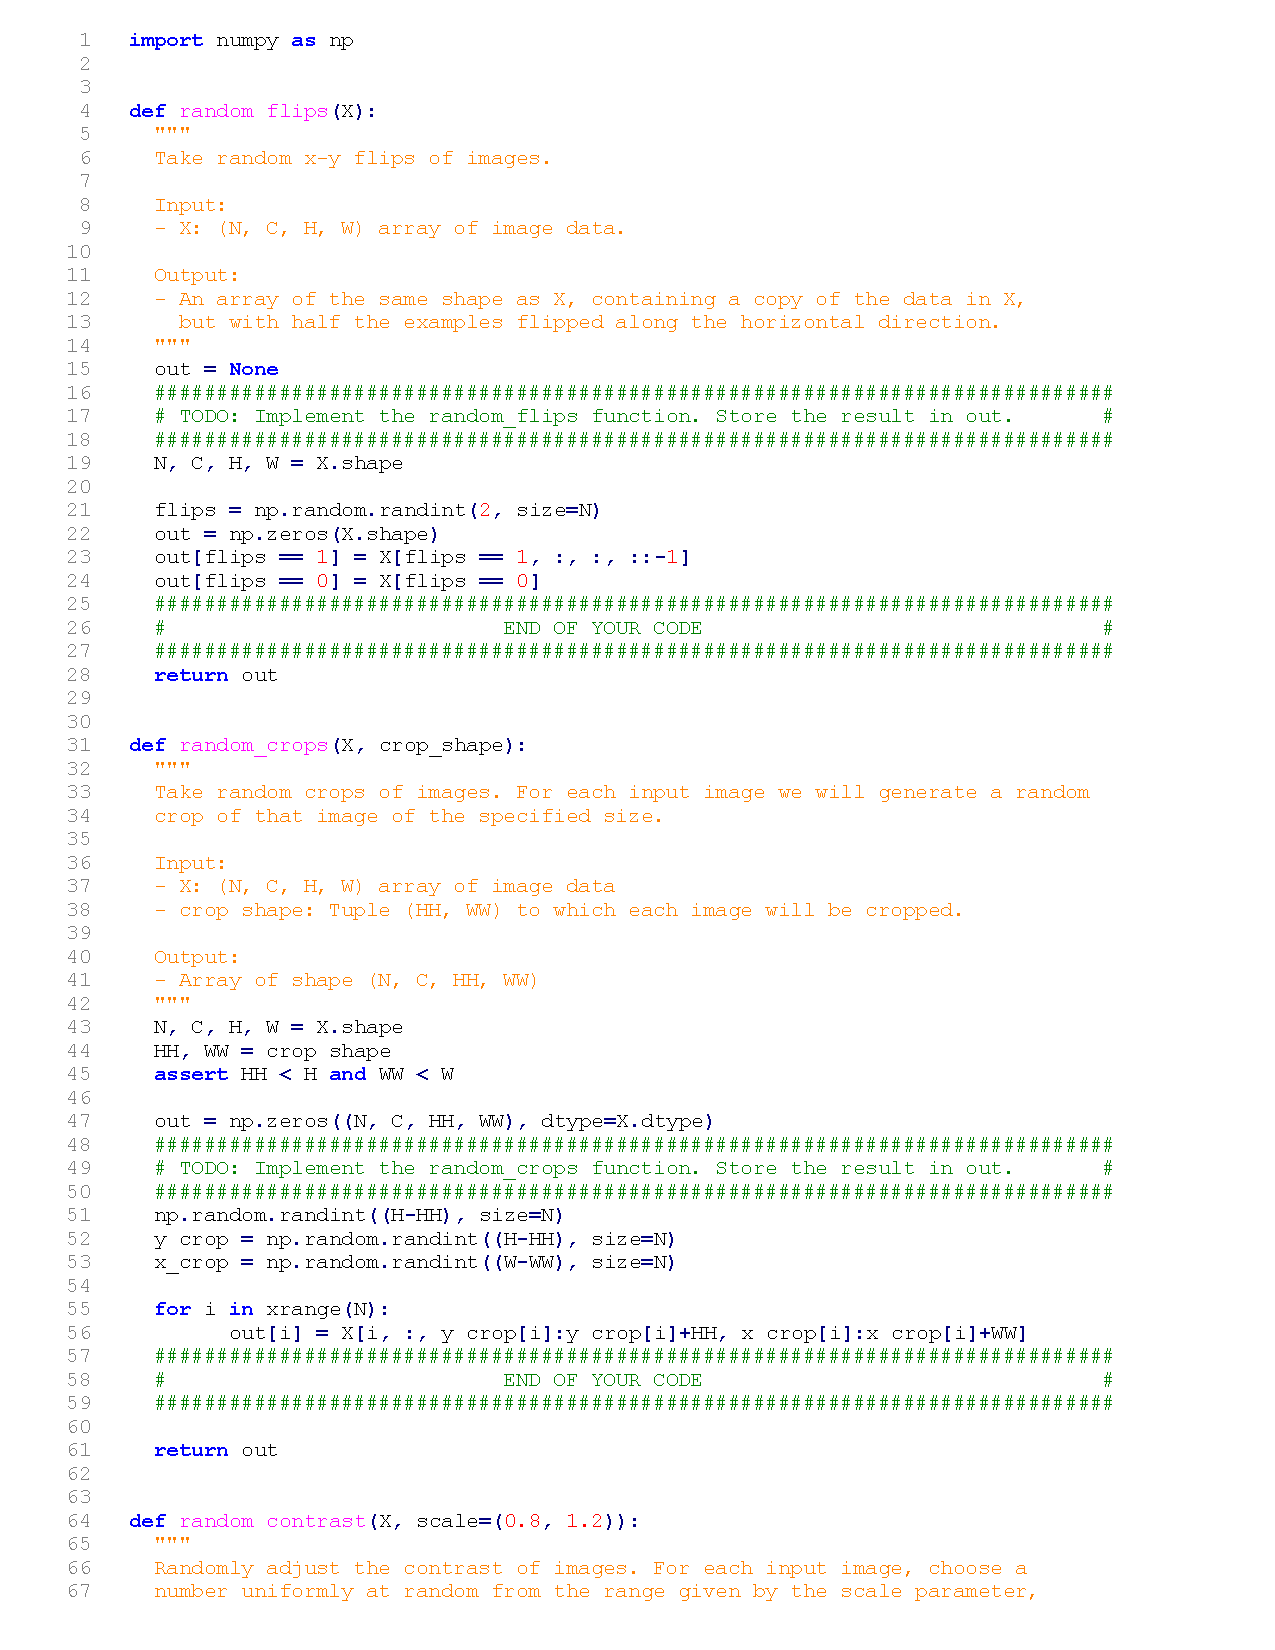
\includepdf[pages=-]{../chapter/appendix/Exercise2/data_augmentation}
\end{appendices}